\documentclass[12pt]{article}
\usepackage[a4paper, total={6in, 10in}]{geometry}
\usepackage{graphicx}
\graphicspath{{figs/}} 


\title{Human-Humanoid Dance Demo for OpenDay} 
\author{Miguel P Xochicale \\ 
School of Engineering \\
University of Birmingham
}
\date{June 2018}

\begin{document}
\maketitle
%\thispagestyle{empty} %No number


\begin{abstract}
Document for a brief description of the demonstration of a human-humanoid 
interaction activity at the Open Day of The University of Birmingham.
\end{abstract}

%\section{Introduction}
For the demo, NAO, a humanoid robot \cite{gouaillier2008} has been programmed 
to move their arms from left to right in a continues way (Fig \ref{fig:nao}).
Additionally, the velocity for NAO's arm movement repetition changed from slow to faster 
and then slow down as show in Fig \ref{fig:armangles}.
In the experiment, participants were asked to wear inertial measurement units
and with a webcam, video were recorded to estimate the head pose with Openface framework 
\cite{baltrusaitis2016, baltrusaitis2018}.
Fig \ref{fig:participants} show six participants imitating upper arm movements
performed by NAO. It can be noticed that detecting the face of participant p08 was fine (E)
but when two extra persons were interested in the experiment, and included in the video frame,  
made OpenFace framework to track the head pose estimation of other person (F).


%%---------------------------------(FIGURE)-------------------------------------
\begin{figure}[!ht]
\centering
\includegraphics[width=0.5\textwidth]{nao/naoarms}
    \caption{
	{\bf Nao.}
	 Upper arm movements of NAO.
        }
\label{fig:nao}
\end{figure}
%%---------------------------------(FIGURE)------


%%---------------------------------(FIGURE)-------------------------------------
\begin{figure}[!ht]
\centering
\includegraphics[width=1.0\textwidth]{nao/lrarms}
    \caption{
	{\bf Joint angles of NAO.}
	Time series show the increase and decrease of frequency 
	of the join angles for (A) Left arm, and (B) right arm. 
        }
\label{fig:armangles}
\end{figure}
%%---------------------------------(FIGURE)------



%%---------------------------------(FIGURE)-------------------------------------
\begin{figure}[!ht]
\centering
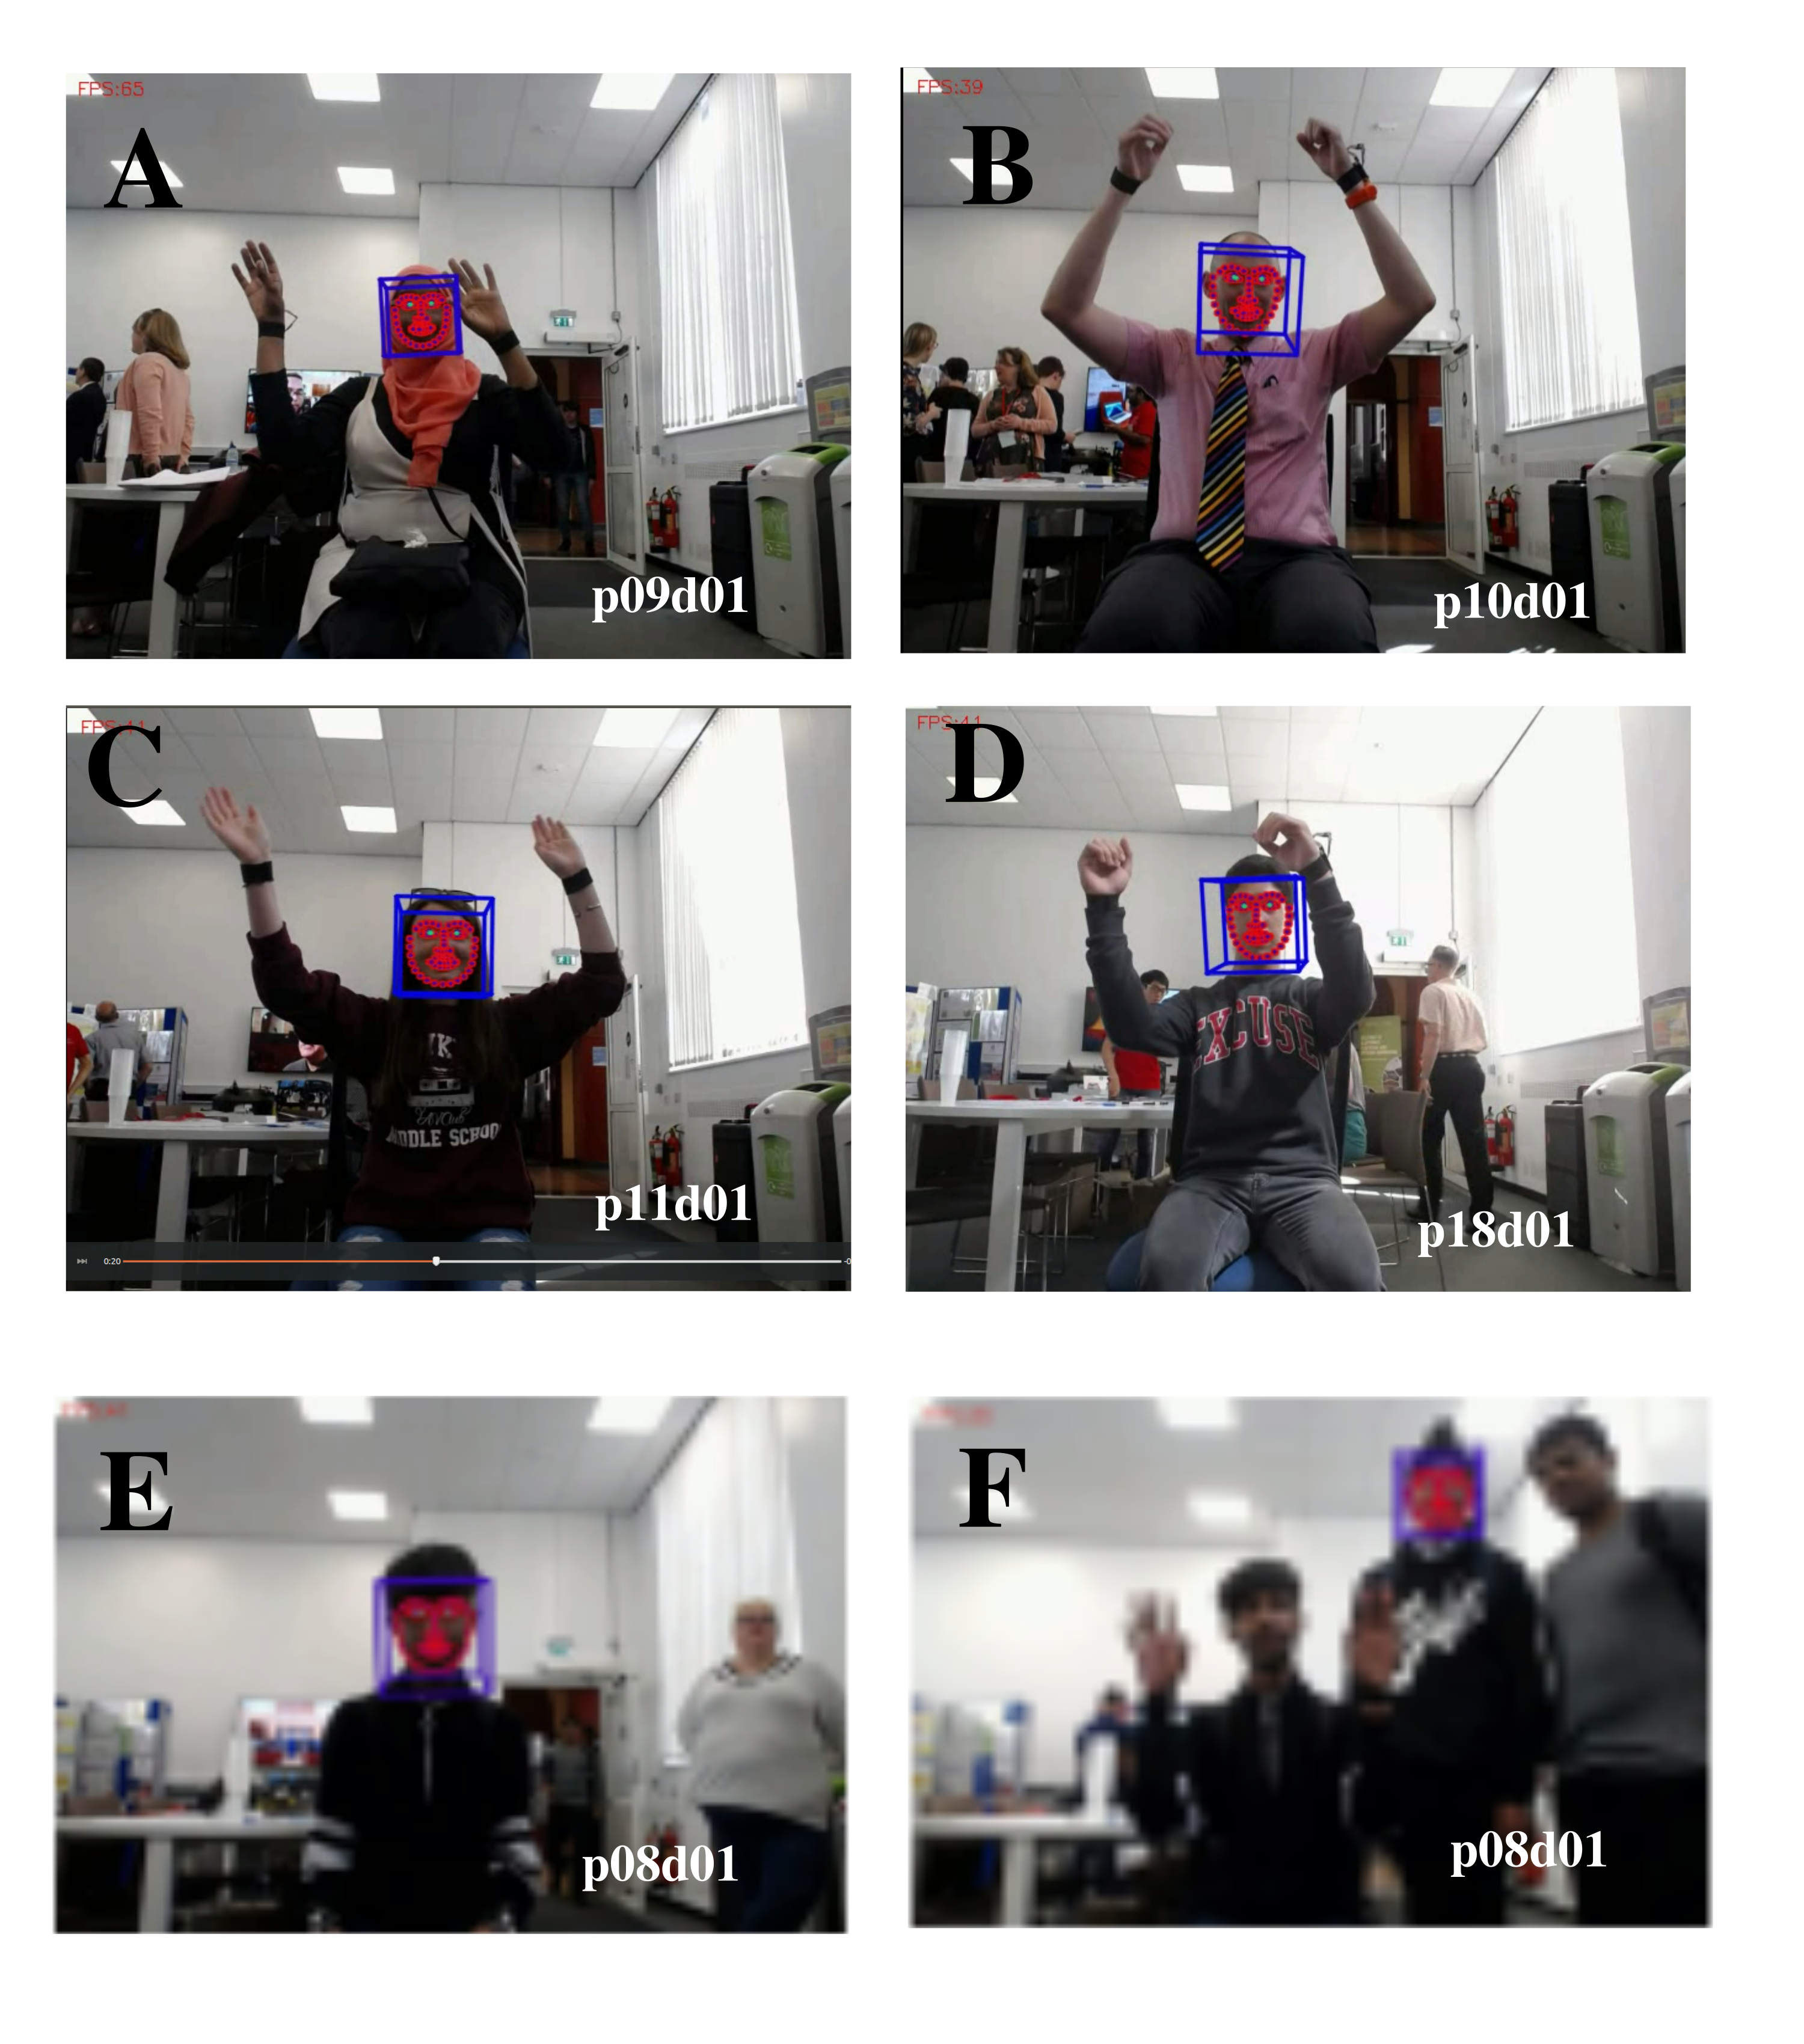
\includegraphics[width=1.0\textwidth]{participants/participants}
    \caption{
	{\bf Six participants performing the Human-Humanoid Imitation Demo.}
	The head pose estimation is presented for each of the participants (A-F).
	Detecting the face of participant p08 was fine (E), however, two extra persons 
	were interested in the experiment of (E) which made OpenFace framework 
	to track the head pose estimation of other person (F).
        }
\label{fig:participants}
\end{figure}
%%---------------------------------(FIGURE)------





\newpage

\bibliographystyle{apalike}
\bibliography{references/references}





\end{document}
